In this exercise, we compare two expert algorithms, \textbf{Follow the Leader (FTL)} and \textbf{Hedge}, for predicting a binary sequence. We measure performance by the (pseudo)regret or regret against the best constant expert in hindsight. The code is contained in the file \texttt{FTL\_and\_Hedge.py}, and it tests both an i.i.d.\ Bernoulli setting (varying \(\mu\)) and an adversarial setting designed to challenge FTL.

\subsection*{1) Implementation, Code Snippets, and i.i.d.\ Results}

\paragraph{Key Code Snippets.}
Below are the core parts of the implementation.  First, the \textbf{FTL} algorithm:

\begin{lstlisting}[language=Python, caption={FTL implementation.}]
def ftl_predict(X):
    T = len(X)
    cum_loss = np.zeros(T)
    L0, L1 = 0, 0
    mistakes = 0
    for t in range(T):
        # Choose the leader (expert with fewer mistakes)
        if L0 < L1:
            pred = 0
        elif L1 < L0:
            pred = 1
        else:
            pred = 0  # tie-breaker

        # Check if we made a mistake
        if pred != X[t]:
            mistakes += 1

        # Update the experts' mistakes
        if X[t] == 1:
            L0 += 1
        else:
            L1 += 1

        cum_loss[t] = mistakes
    return cum_loss
\end{lstlisting}

Then, the \textbf{Hedge} algorithm with two experts (always predict~0 or always predict~1).  The parameter \(\eta\) (learning rate) can be \emph{fixed} or \emph{anytime}:

\begin{lstlisting}[language=Python, caption={Hedge implementation.}]
def hedge_predict(X, schedule_type, param):
    T = len(X)
    L = np.zeros(2)  # losses for expert0 and expert1
    cum_loss = np.zeros(T)
    mistakes = 0
    for t in range(1, T+1):
        # Define eta_t
        if schedule_type == 'fixed':
            eta_t = param
        else:  # 'anytime'
            eta_t = param * np.sqrt(np.log(2)/t)

        # Exponential weights
        L_min = np.min(L)
        w = np.exp(-eta_t * (L - L_min))
        p = w / np.sum(w)

        # Sample prediction
        action = np.random.choice([0,1], p=p)
        if action != X[t-1]:
            mistakes += 1

        # Update experts' losses
        loss0 = 1 if X[t-1] == 1 else 0
        loss1 = 1 if X[t-1] == 0 else 0
        L[0] += loss0
        L[1] += loss1

        cum_loss[t-1] = mistakes
    return cum_loss
\end{lstlisting}

Finally, for each i.i.d.\ experiment, we run these algorithms on 10 independent Bernoulli(\(\mu\)) sequences of length \(T=2000\), compute each algorithm's cumulative loss, and subtract the best constant expert's loss to obtain the \emph{pseudo-regret}.

\paragraph{Numeric Values of Hedge Parameters.}
In the output, there are names like \texttt{Hedge\_fixed(0.0263)}.  The number in parentheses is the numeric value of \(\eta\).  We use the following formulas (with \(T=2000\) and \(\ln(2)\approx 0.693\)):

\begin{itemize}
\item \(\eta = \sqrt{\frac{2\ln(2)}{T}}\approx 0.0263\)
\item \(\eta = \sqrt{\frac{8\ln(2)}{T}}\approx 0.0527\)
\item For anytime Hedge: \(\eta_t = c \sqrt{\frac{\ln(2)}{t}}\) with \(c \in \{1,2\}\).
\end{itemize}

\begin{table}[h!]
\centering
\begin{tabular}{lll}
\hline
\textbf{Algorithm Name} & \textbf{Formula} & \textbf{Value for $T=2000$}\\
\hline
\texttt{Hedge\_fixed(0.0263)} & $\sqrt{2\ln(2)/T}$ & $0.0263$ \\
\texttt{Hedge\_fixed(0.0527)} & $\sqrt{8\ln(2)/T}$ & $0.0527$ \\
\texttt{Hedge\_anytime(1.0)}  & $1.0\sqrt{\ln(2)/t}$ & \emph{varies with $t$} \\
\texttt{Hedge\_anytime(2.0)}  & $2.0\sqrt{\ln(2)/t}$ & \emph{varies with $t$} \\
\hline
\end{tabular}
\caption{Correspondence between Hedge formulas and the displayed numeric parameters.}
\label{tab:hedge_values}
\end{table}

\paragraph{Outputs and Plots (i.i.d.\ Setting).}
Below are the final average pseudo-regrets for \(\mu=0.25, 0.375, 0.4375\).  Each block corresponds to 10 runs, each of length \(T=2000\):

\begin{verbatim}
Final average pseudo-regret at t=2000 for p=0.25:
  FTL: 0.200
  Hedge_fixed(0.026327688477341595): 26.000
  Hedge_fixed(0.05265537695468319): 13.400
  Hedge_anytime(1.0): 4.600
  Hedge_anytime(2.0): 1.400
--------------------------------------------------

Final average pseudo-regret at t=2000 for p=0.375:
  FTL: 1.800
  Hedge_fixed(0.026327688477341595): 26.800
  Hedge_fixed(0.05265537695468319): 15.500
  Hedge_anytime(1.0): 13.800
  Hedge_anytime(2.0): 5.700
--------------------------------------------------

Final average pseudo-regret at t=2000 for p=0.4375:
  FTL: 5.100
  Hedge_fixed(0.026327688477341595): 29.700
  Hedge_fixed(0.05265537695468319): 13.100
  Hedge_anytime(1.0): 20.300
  Hedge_anytime(2.0): 11.700
\end{verbatim}

Figures~\ref{fig:plot_mu025}, \ref{fig:plot_mu0375}, and \ref{fig:plot_mu04375} show the pseudo-regret curves over time for the three values of \(\mu\).  

\begin{figure}[H]
\centering
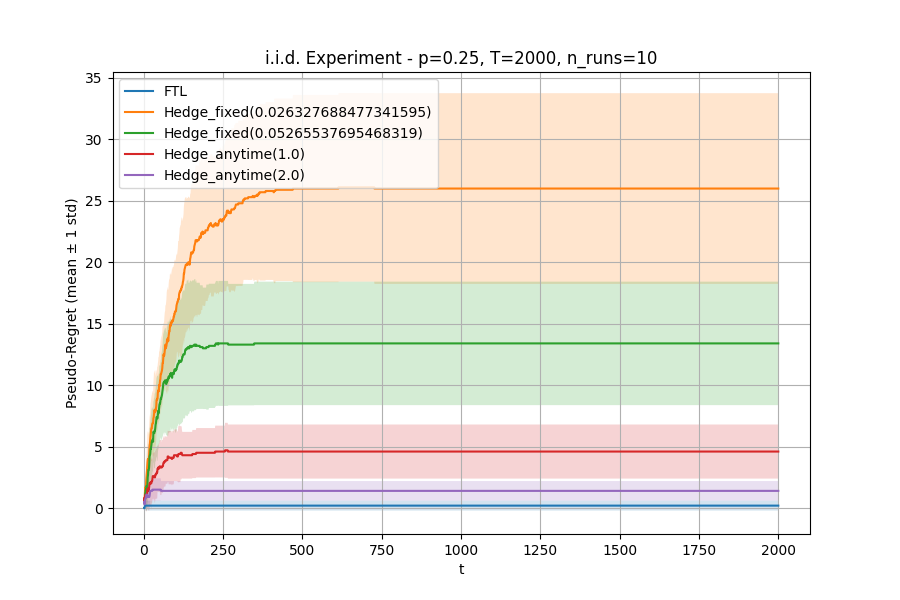
\includegraphics[width=0.85\textwidth]{Code/plot_iid_025.png}
\caption{Pseudo-regret for \(\mu=0.25\).}
\label{fig:plot_mu025}
\end{figure}

\begin{figure}[H]
\centering
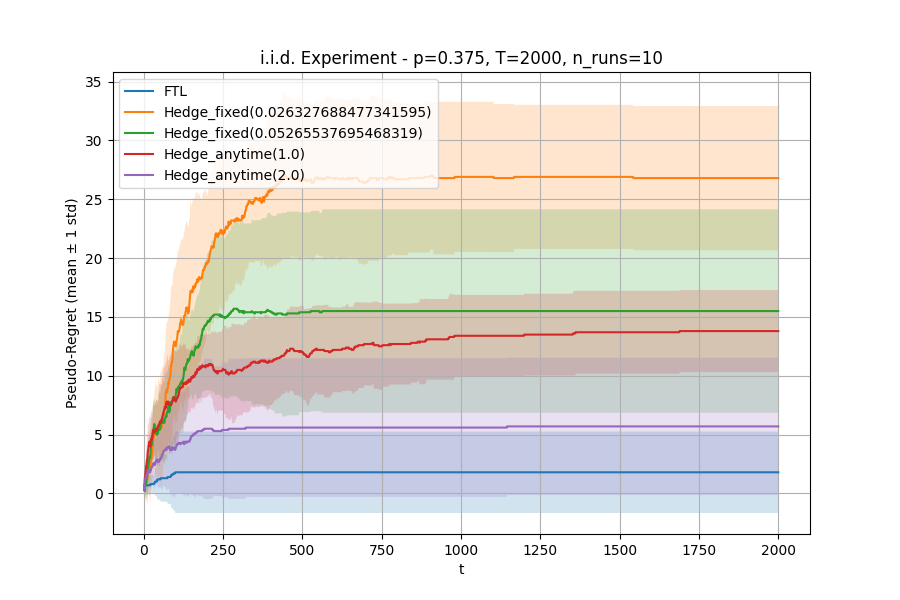
\includegraphics[width=0.85\textwidth]{Code/plot_iid_0375.png}
\caption{Pseudo-regret for \(\mu=0.375\).}
\label{fig:plot_mu0375}
\end{figure}

\begin{figure}[H]
\centering
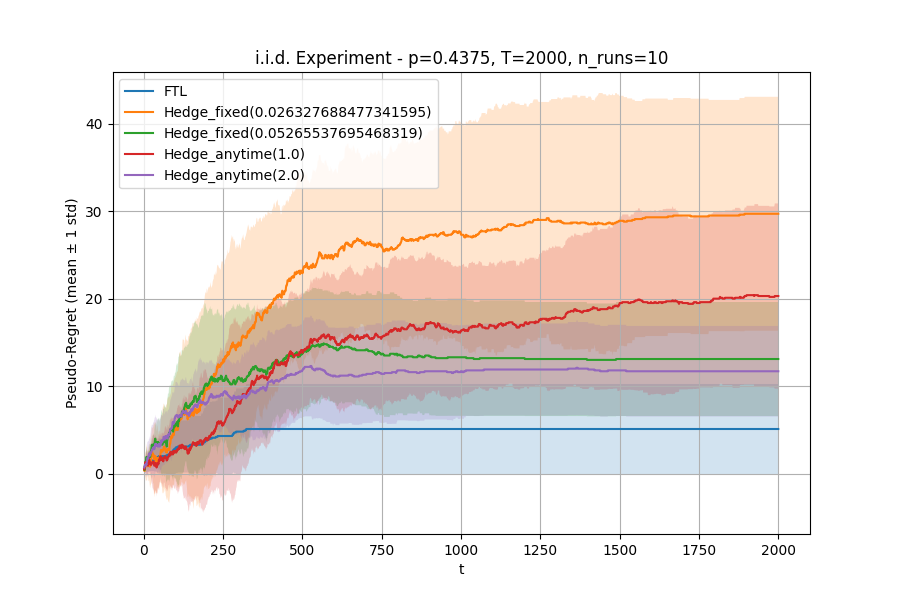
\includegraphics[width=0.85\textwidth]{Code/plot_iid_04375.png}
\caption{Pseudo-regret for \(\mu=0.4375\).}
\label{fig:plot_mu04375}
\end{figure}

\subsection*{2) Influence of \texorpdfstring{$\mu$}{mu} and Performance Over Time}

\textbf{Which values of \(\mu\) lead to higher regret?}  
The results indicate that when \(\mu\) is closer to 0.5, the pseudo-regret tends to be higher. This is because when the distribution is more balanced, the difference between the mistakes of the constant experts (always predicting 0 or 1) becomes smaller, making it harder for the algorithms to quickly identify a clear majority, which in turn delays convergence and results in higher cumulative pseudo-regret.

\textbf{Does the relative performance evolve with time?}  
Yes. Over time, all algorithms tend to slow down the growth of their pseudo-regret as they collect more samples and better estimate the underlying distribution. In particular, once a sufficient number of observations have been collected, the algorithms' pseudo-regret curves start to plateau. Moreover, for smaller \(\mu\) (i.e., when the distribution is more skewed), this plateau is reached earlier since the dominant class becomes apparent sooner. Conversely, when \(\mu\) is closer to 0.5, it takes longer for the algorithms to settle, resulting in a slower reduction of the pseudo-regret growth rate.

\subsection*{3) Adversarial Case and Its Effect on FTL}

We now consider an adversarial sequence.  We define:

\begin{lstlisting}[language=Python, caption={Adversarial sequence alternating 0 and 1.}]
def simulate_adversarial_sequence(T):
    return np.array([t % 2 for t in range(1, T+1)])
\end{lstlisting}

In this case, we measure \emph{regret} (algorithm’s cumulative loss minus the best constant expert’s loss).  The final average regret at \(t=2000\) over 10 runs is:

\begin{verbatim}
Final average regret at t=2000 (adversarial):
  FTL: 1000.000
  Hedge_fixed(0.026327688477341595): -3.200
  Hedge_fixed(0.05265537695468319): 29.900
  Hedge_anytime(1.0): 16.200
  Hedge_anytime(2.0): 13.500
\end{verbatim}

\noindent
Figure~\ref{fig:plot_adversarial} shows the regret over time.  We observe that \textbf{FTL} suffers heavily, reaching a regret of around 1000 by \(t=2000\).  Meanwhile, some Hedge variants maintain very low or even negative regret (meaning they do better than the best constant expert).

\begin{figure}[H]
\centering
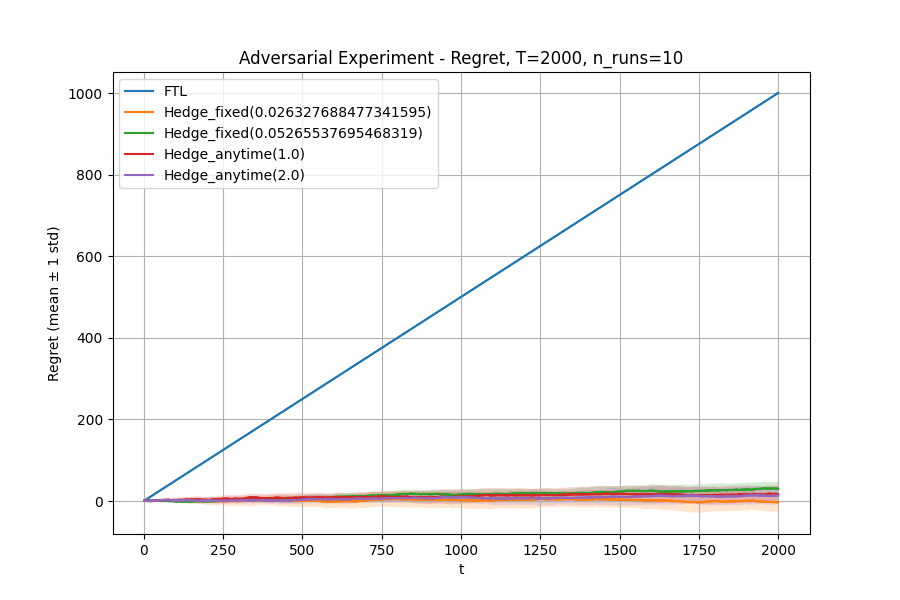
\includegraphics[width=0.85\textwidth]{Code/plot_adversarial_example.png}
\caption{Regret over time on the adversarial sequence (alternating 0,1).}
\label{fig:plot_adversarial}
\end{figure}

These results highlight that FTL can be outperformed by Hedge in adversarial scenarios.  The exact extent depends on the learning rate choice, but \texttt{Hedge\_anytime(1.0)} and \texttt{Hedge\_anytime(2.0)} generally avoid large regret growth.

\bigskip
\noindent
\textbf{Note:} All code and further details can be found in \texttt{FTL\_and\_Hedge.py}. That can be run to replicate these experiments.
